\documentclass[11pt]{article}

% Load fontspec package to set the font with LuaLaTeX
% \usepackage{fontspec}

% Set the main font to Courier New
% \setmainfont{Courier New}

\usepackage[margin = 0.75in]{geometry}
\geometry{letterpaper}

\usepackage{graphicx}
\usepackage{amssymb, amsmath}
\usepackage{breqn}
\usepackage{epstopdf}
\usepackage{enumerate}
\usepackage{algorithm}
\usepackage{algpseudocode}
\usepackage{listings}
\usepackage{indentfirst}
\usepackage{xcolor}
\usepackage[T1]{fontenc}
\usepackage{subcaption}


\definecolor{codebg}{rgb}{0.95,0.95,0.95}
\definecolor{keywordcolor}{rgb}{0.0,0.0,0.6}
\definecolor{stringcolor}{rgb}{0.58,0,0.03}
\definecolor{commentcolor}{rgb}{0.0,0.5,0.0}

\lstdefinelanguage{Python}{
    keywords={def, return, if, elif, else, while, for, in, try, except, finally, raise, import, from, as, pass, class, break, continue, with, lambda, assert, yield, True, False, None, and, or, not, is},
    keywordstyle=\color{keywordcolor}\bfseries,
    ndkeywords={self},
    ndkeywordstyle=\color{black},
    identifierstyle=\color{black},
    sensitive=true,
    comment=[l]\#,
    commentstyle=\color{commentcolor}\ttfamily,
    stringstyle=\color{stringcolor},
    morestring=[b]',
    morestring=[b]",
    morecomment=[s]{"""}{"""},
    morecomment=[s]{'''}{'''},
}

\lstset{
    language=Python,
    backgroundcolor=\color{codebg},
    basicstyle=\ttfamily\footnotesize,
    frame=single,
    showstringspaces=false,
    tabsize=4,
    captionpos=b,
    breaklines=true,
    breakatwhitespace=true,
    numbers=left,
    numberstyle=\tiny\color{gray},
}

\DeclareGraphicsRule{.tif}{png}{.png}{convert #1 dirname #1/basename #1 .tif.png}
\graphicspath{{./figures/}}

% Setup IEEE BibLaTeX style
\usepackage[backend=biber, style=ieee]{biblatex}

% Setup Footer
\usepackage{fancyhdr}
\pagestyle{fancy}

\begin{document} 


\begin{titlepage}
    \begin{center}
        \vspace*{1cm}

        \textbf{AE5093 — Scientific Applications of Deep Learning}

        \vspace{0.5cm}
            Homework 4
                
        \vspace{1.5cm}

        \textbf{Daniel J. Pearson}

        \vfill
                
        \vspace{0.8cm}
        
        
\includegraphics[width=0.4\textwidth]{WPI_LOGO}

        % \includegraphics[width=0.4\textwidth]{university}
                
        Aerospace Engineering Department\\
        Worcester Polytechnic Institute\\
        \date{\today}
                
    \end{center}
\end{titlepage}

\pagebreak

\section{Introduction}
In this assigment, a Feed Forward Neural Network (FFNN) is trained and informed using a physical model of a system. The network will be trained on two PDEs: the 1D viscous Burgers equation and the 2D wave equation. The goal is to demonstrate the ability of the FFNN to learn the underlying physics of the system and make predictions based on the model. For both cases, it will be fed a series of boundary conditions and interior points to learn. 

\section{1D Burgers Equation}
The 1D viscous Burgers equation is a fundamental partial differential equation (PDE) that describes the motion of a viscous fluid. It is given by:
\begin{equation}
    u_t + u*u_x = \nu u_{xx}
\end{equation}

where $u$ is the velocity field, $t$ is time, $x$ is the spatial coordinate, and $\nu$ is the kinematic viscosity.

\subsection{Problem Setup}
For this problem, the domain is defined as $x \in [-1, 1]$ and $t \in [0, 1]$. With the following boundary conditions:
\begin{equation}
    u(x, 0) = -\sin(\pi x)
\end{equation}
\begin{equation}
    u(-1, t) = u(1,t) = 0
\end{equation}
 
where,
\[
\nu \in \lbrace \frac{0.01}{\pi}, \frac{0.0001}{\pi}, 0.0 \rbrace
\].

For each viscous case, the following parameters are used:
\begin{itemize}
    \item Epochs = 5000
    \item LearningRate = 1000
    \item Neurons = 50
    \item $N_{i}  = 5000$ (interior points)
    \item $N_{b}  = 256$  (boundary points)
    \item $N_{ic} = 256$  (initial condition points)
\end{itemize}

The NN will be trained on the interior points, boundary points and initial conditions. The total loss function is defined by:
\begin{equation}
    L = L_{pde} + L_{ic} + L_{bc}
\end{equation}
where,
\begin{equation}
    L_{pde} = u_t + u u_x - \nu u_{xx}
\end{equation}
\begin{equation}
    L_{ic} = \frac{1}{N} \sum_{i=1}^{N} (\theta(u|x_{ic}, t_{ic})-u_{ic})^2
\end{equation}
\begin{equation}
    L_{bc} = L_{ic} = \frac{1}{N} \sum_{i=1}^{N} (\theta(u|x_{bc}, t_{bc})-u_{bc})^2
\end{equation}

\subsection{Results - No LR Annealing}
\subsubsection{Case 1: High Viscosity}
\begin{figure}[h!]
    \centering
    \begin{subfigure}[b]{0.48\textwidth}
        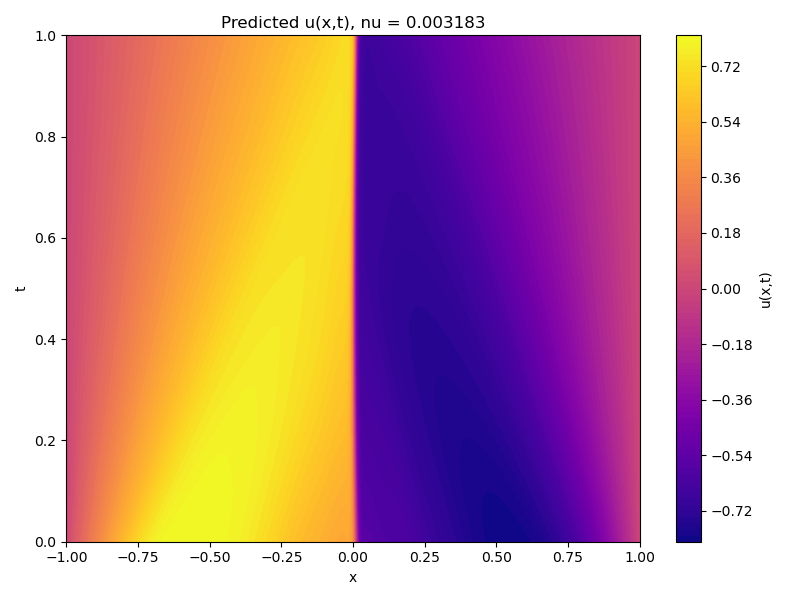
\includegraphics[width=\textwidth]{1D_PredGrad_NU1.png}
        \caption{Prediction Gradient for Case 1: High Viscosity}
        \label{fig:PredGrad_NU1}
    \end{subfigure}
    \hfill
    \begin{subfigure}[b]{0.48\textwidth}
        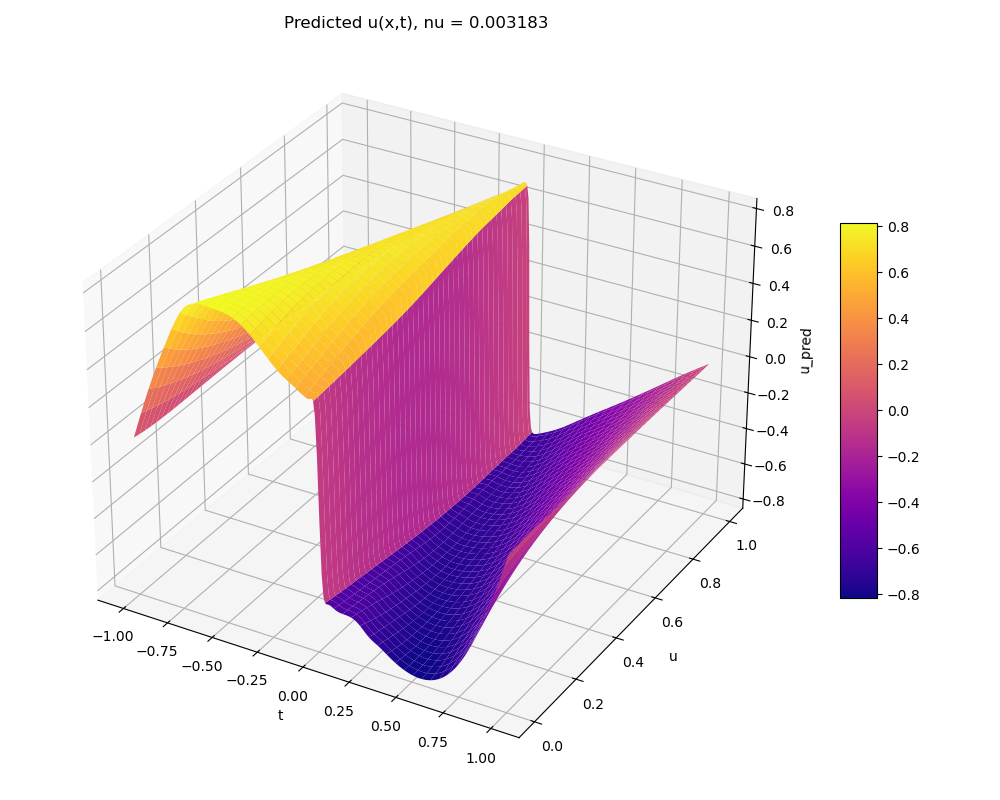
\includegraphics[width=\textwidth]{1D_Pred_NU1.png}
        \caption{Prediction for Case 1: High Viscosity}
        \label{fig:Pred_NU1}
    \end{subfigure}
    \caption{Prediction for Case 1: High Viscosity}
    \label{fig:PredTotal_NU1}
\end{figure}

\begin{figure}[h]
    \centering
    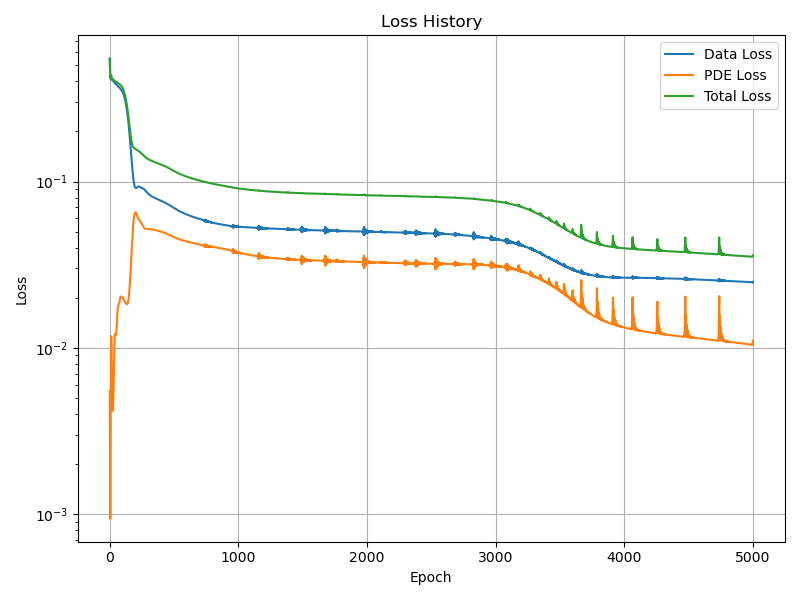
\includegraphics[width=0.6\textwidth]{1D_Loss_NU1.png}
    \caption{Loss for Case 1: High Viscosity}
    \label{fig:Loss_NU1}
\end{figure}

For the first case, the FFNN was trained on the highest viscocity case. The loss function converged to a value of $10^-1.4$ after approximately 4500 epochs. The prediction gradient and 3d plot of the prediction are shown in Figure \ref{fig:PredTotal_NU1}. Since this function does not have a closed form solution, the prediction is compared to a numerical solution. Using the gradient, it is clear that the boundary and initial conditions are satisfied and is a smooth and continuous function expected for a viscous fluid. This case is the most difficult to learn, as the viscocity is high and there is a signfiicant jump discontinuity in the solution.

\pagebreak
\subsubsection{Case 2: Low Viscosity}
\begin{figure}[h!]
    \centering
    \begin{subfigure}[b]{0.48\textwidth}
        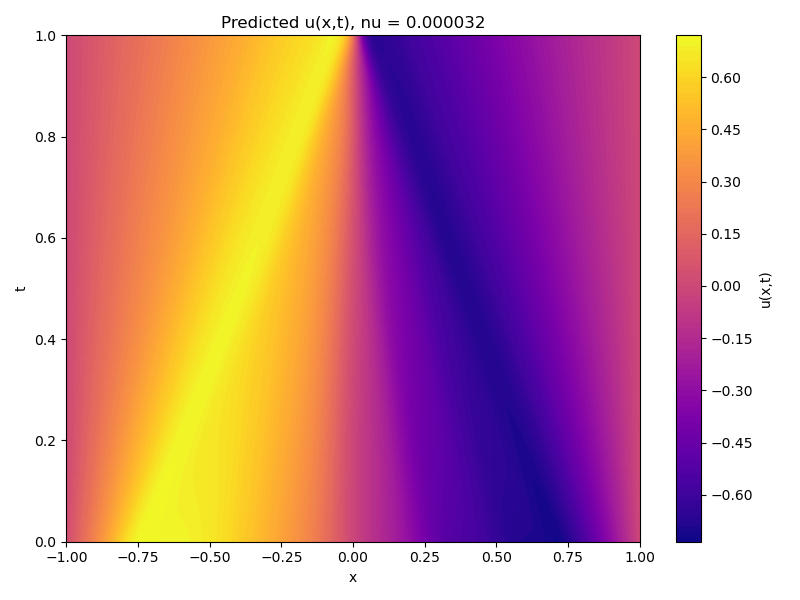
\includegraphics[width=\textwidth]{1D_PredGrad_NU2.png}
        \caption{Prediction Gradient for Case 2: Low Viscosity}
        \label{fig:PredGrad_NU2}
    \end{subfigure}
    \hfill
    \begin{subfigure}[b]{0.48\textwidth}
        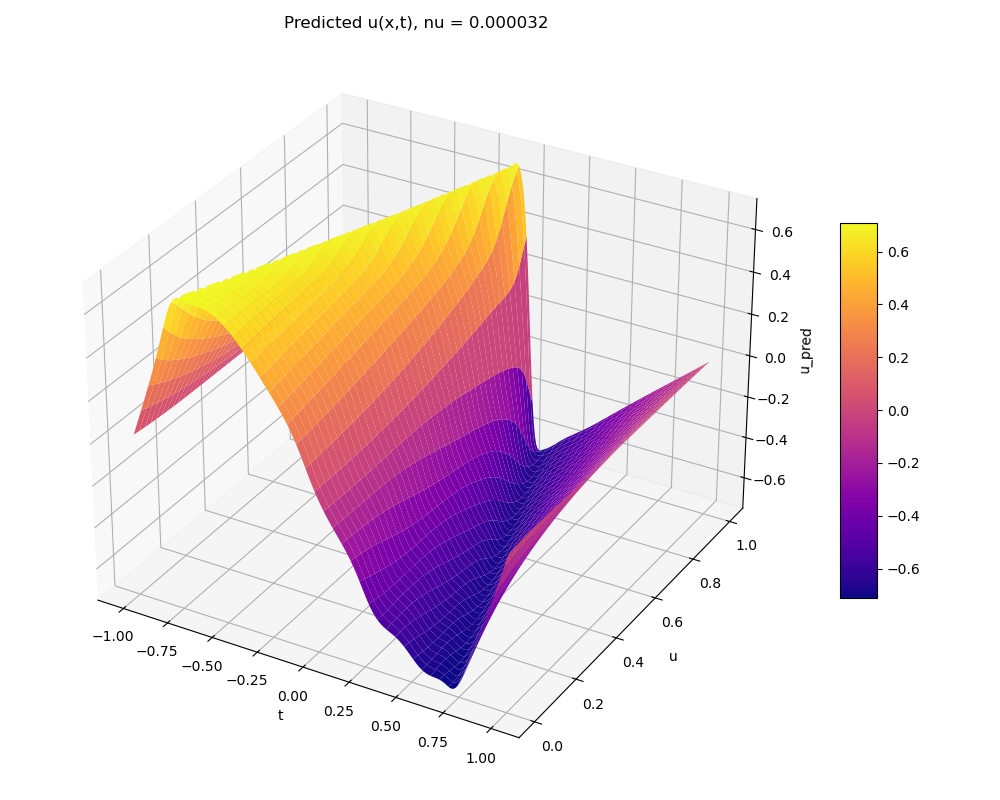
\includegraphics[width=\textwidth]{1D_Pred_NU2.png}
        \caption{Prediction for Case 2: Low Viscosity}
        \label{fig:Pred_NU2}
    \end{subfigure}
    \caption{Prediction for Case 2: Low Viscosity}
    \label{fig:PredTotal_NU2}
\end{figure}

\begin{figure}[h]
    \centering
    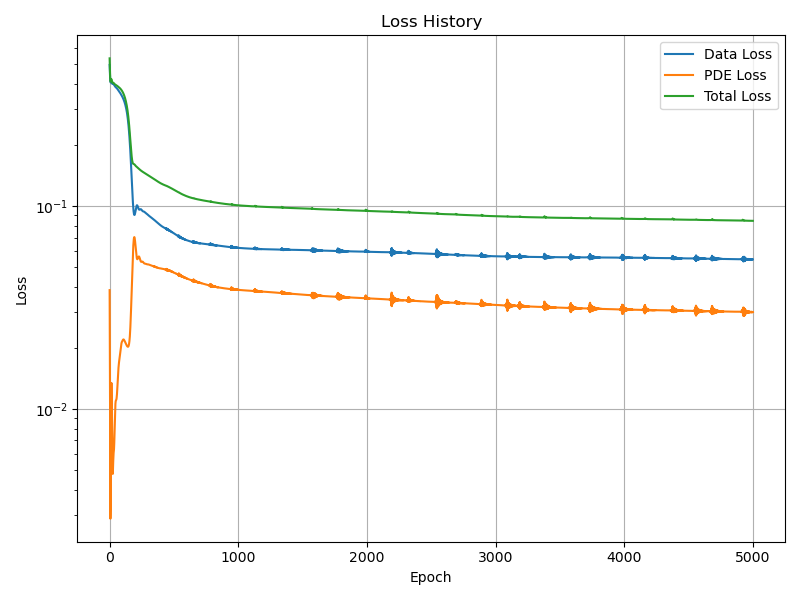
\includegraphics[width=0.6\textwidth]{1D_Loss_NU2.png}
    \caption{Loss for Case 2: Low Viscosity}
    \label{fig:Loss_NU2}
\end{figure}
For the second case, the FFNN was trained on the low viscocity case. The loss function converged to a value of $10^-1.2$ after approximately 3000 epochs. The prediction gradient and 3d plot of the prediction are shown in Figure \ref{fig:PredTotal_NU2}. The prediction is much smoother than the first case and does not have a jump discontinuity. This case is expected to be easier to learn, despite a higher total loss. 

\pagebreak 

\subsubsection{Case 3: No Viscosity}
\begin{figure}[h!]
    \centering
    \begin{subfigure}[b]{0.48\textwidth}
        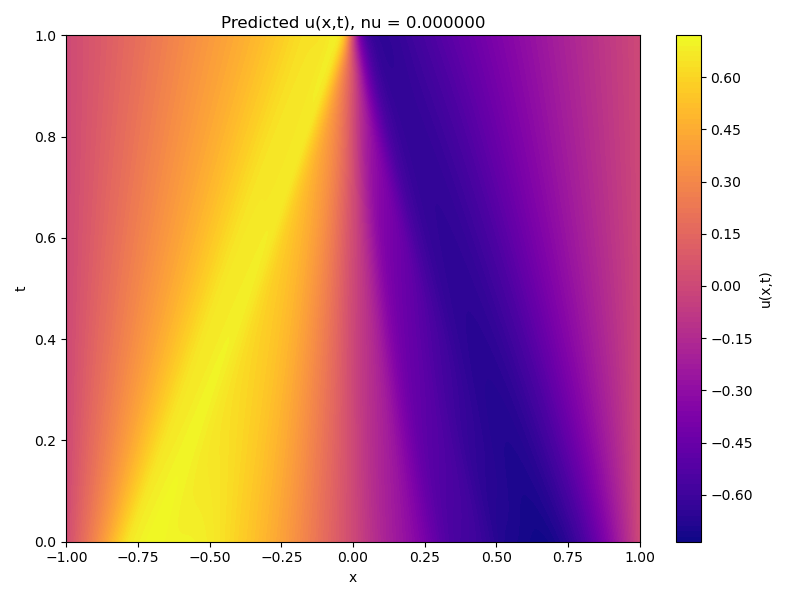
\includegraphics[width=\textwidth]{1D_PredGrad_NU3.png}
        \caption{Prediction Gradient for Case 3: No Viscosity}
        \label{fig:PredGrad_NU3}
    \end{subfigure}
    \hfill
    \begin{subfigure}[b]{0.48\textwidth}
        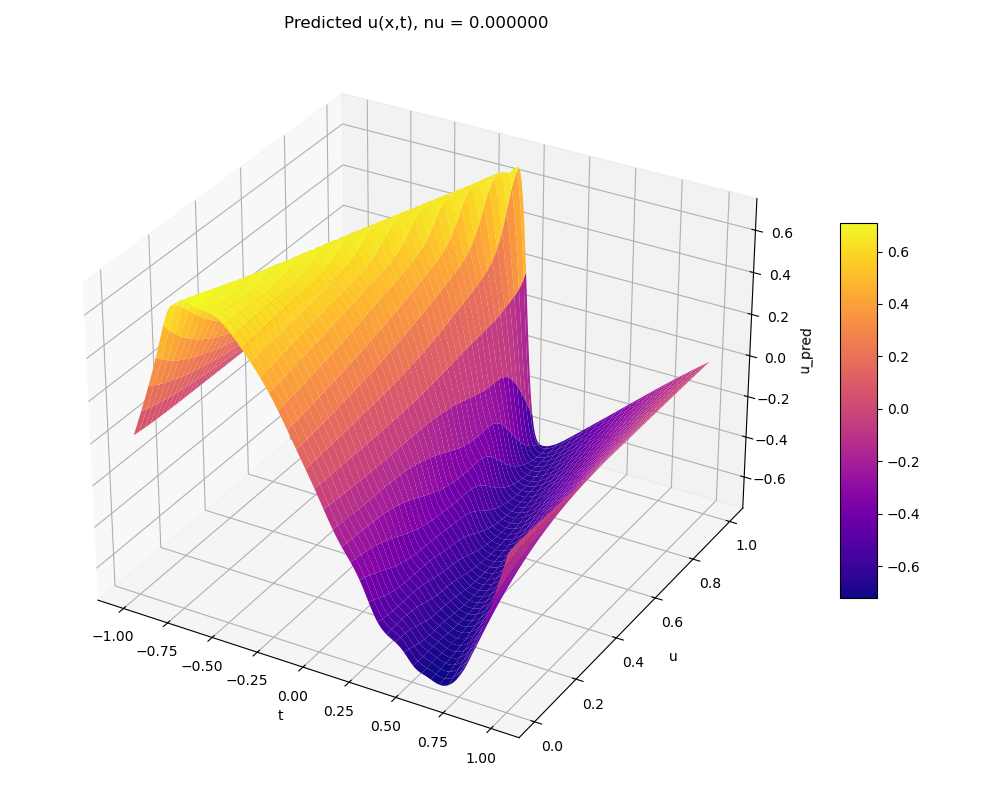
\includegraphics[width=\textwidth]{1D_Pred_NU3.png}
        \caption{Prediction for Case 3: No Viscosity}
        \label{fig:Pred_NU3}
    \end{subfigure}
    \caption{Prediction for Case 3: No Viscosity}
    \label{fig:PredTotal_NU3}
\end{figure}

\begin{figure}[h]
    \centering
    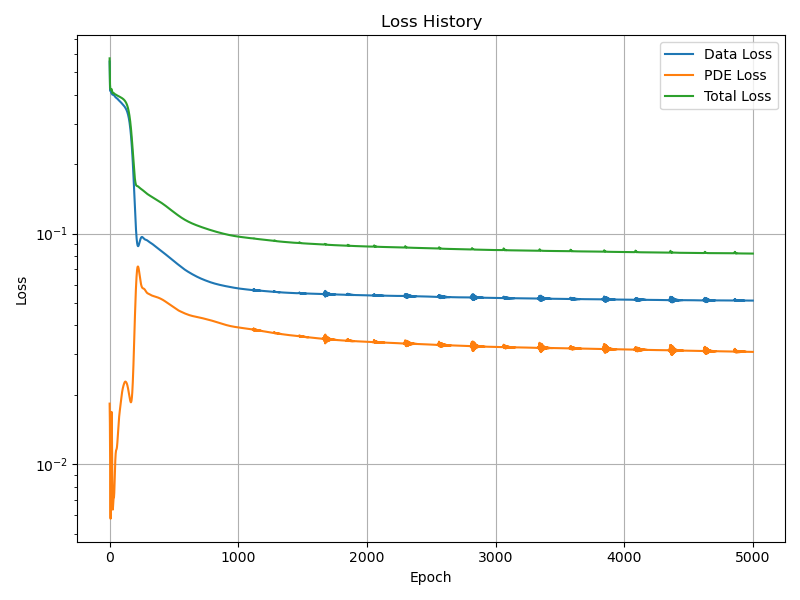
\includegraphics[width=0.6\textwidth]{1D_Loss_NU3.png}
    \caption{Loss for Case 3: No Viscosity}
    \label{fig:Loss_NU3}
\end{figure}

For the third case, the FFNN was trained on the no viscocity case. The loss function converged to a value of $10^-1.2$ after approximately 2000 epochs. The prediction gradient and 3d plot of the prediction are shown in Figure \ref{fig:PredTotal_NU3}. The non-viscous case also matched well with numerical solutions. The prediction is smooth and continous, as expected.
\subsection{Results - LR Annealing}
For the second set of cases, the FFNN was trained with a learning rate annealing approach. Using, $\lambda=0.9$ the following results are obtained.
\subsubsection{Case 1: High Viscosity}
\begin{figure}[h!]
    \centering
    \begin{subfigure}[b]{0.48\textwidth}
        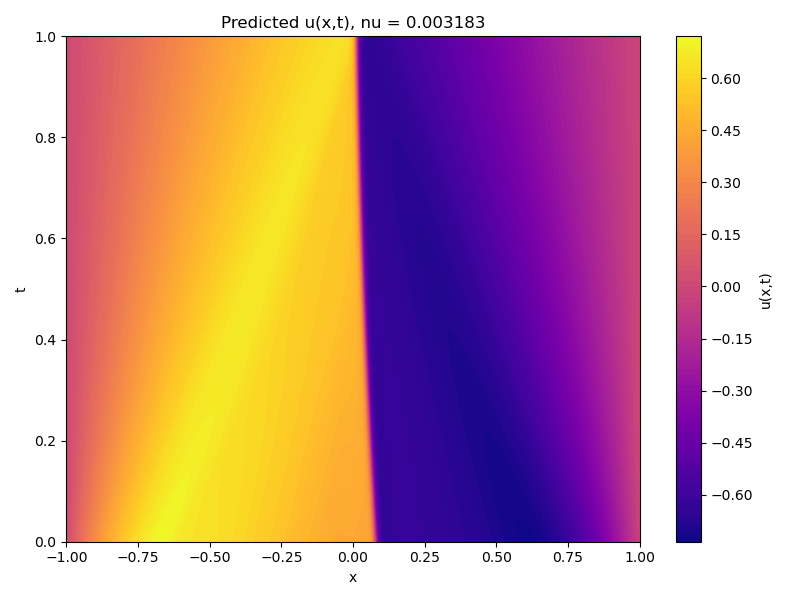
\includegraphics[width=\textwidth]{1D_PredGrad_NU1_Annealing.png}
        \caption{Prediction Gradient for Case 1: High Viscosity}
        \label{fig:PredGrad_NU1_LR}
    \end{subfigure}
    \hfill
    \begin{subfigure}[b]{0.48\textwidth}
        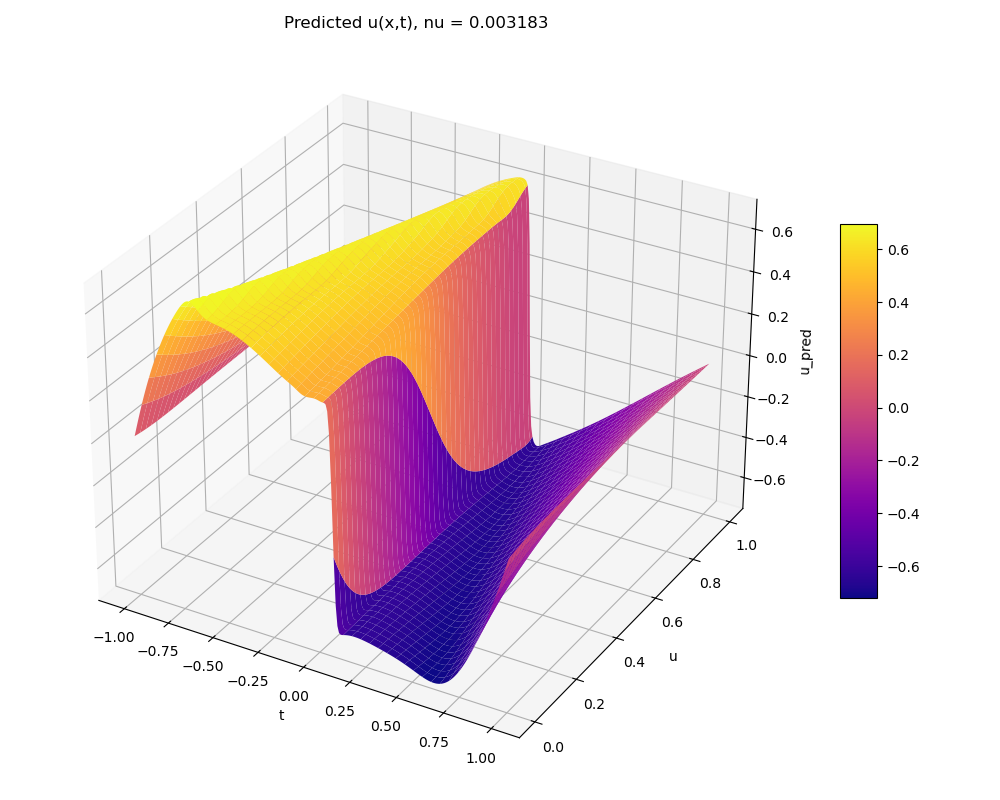
\includegraphics[width=\textwidth]{1D_Pred_NU1_Annealing.png}
        \caption{Prediction for Case 1: High Viscosity}
        \label{fig:Pred_NU1_LR}
    \end{subfigure}
    \caption{Prediction for Case 1: High Viscosity}
    \label{fig:PredTotal_NU1_LR}
\end{figure}
\begin{figure}[h]
    \centering
    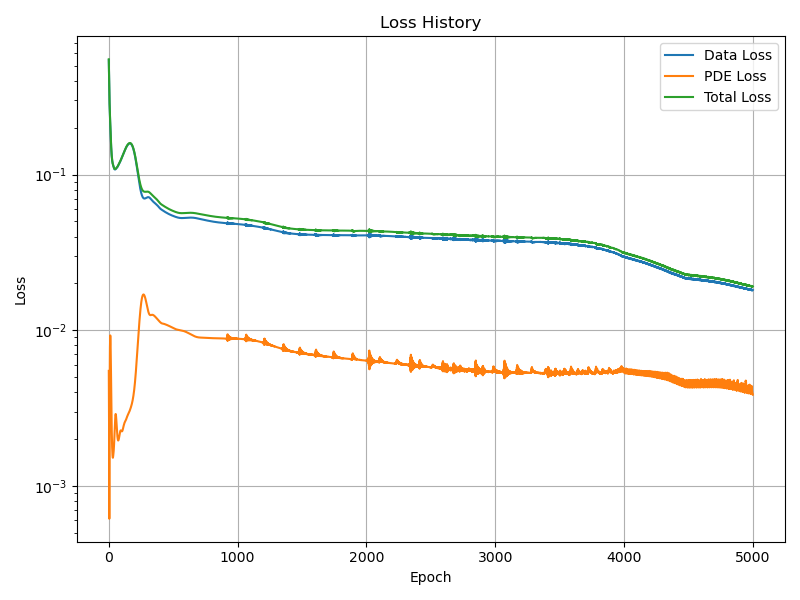
\includegraphics[width=0.6\textwidth]{1D_Loss_NU1_Annealing.png}
    \caption{Loss for Case 1: High Viscosity}
    \label{fig:Loss_NU1_LR}
\end{figure}

Compared to the case without annealing, the FFNN was able to converge to a smoother loss function with the data loss function converging significantly faster and closer to the total loss of $10^-1.7$. The prediction gradient and 3d plot of the prediction are shown in Figure \ref{fig:PredTotal_NU1_LR}. The prediction is much smoother than the first case and still captures the jump discontinuity.

\pagebreak
\subsubsection{Case 2: Low Viscosity}
\begin{figure}[h!]
    \centering
    \begin{subfigure}[b]{0.48\textwidth}
        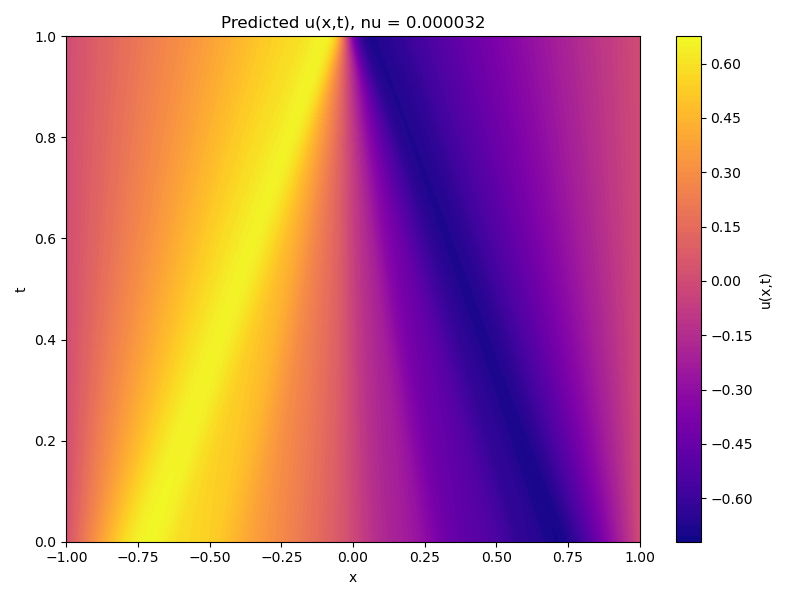
\includegraphics[width=\textwidth]{1D_PredGrad_NU2_Annealing.png}
        \caption{Prediction Gradient for Case 2: Low Viscosity}
        \label{fig:PredGrad_NU2_LR}
    \end{subfigure}
    \hfill
    \begin{subfigure}[b]{0.48\textwidth}
        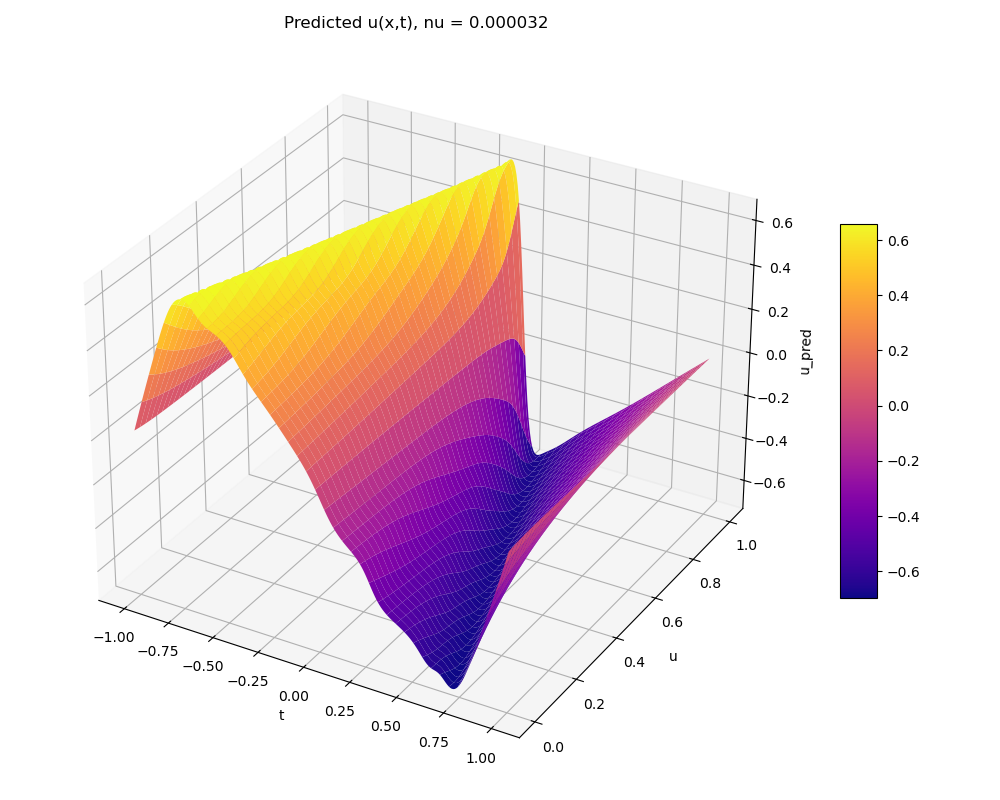
\includegraphics[width=\textwidth]{1D_Pred_NU2_Annealing.png}
        \caption{Prediction for Case 2: Low Viscosity}
        \label{fig:Pred_NU2_LR}
    \end{subfigure}
    \caption{Prediction for Case 2: Low Viscosity}
    \label{fig:PredTotal_NU2_LR}
\end{figure}
\begin{figure}[h]
    \centering
    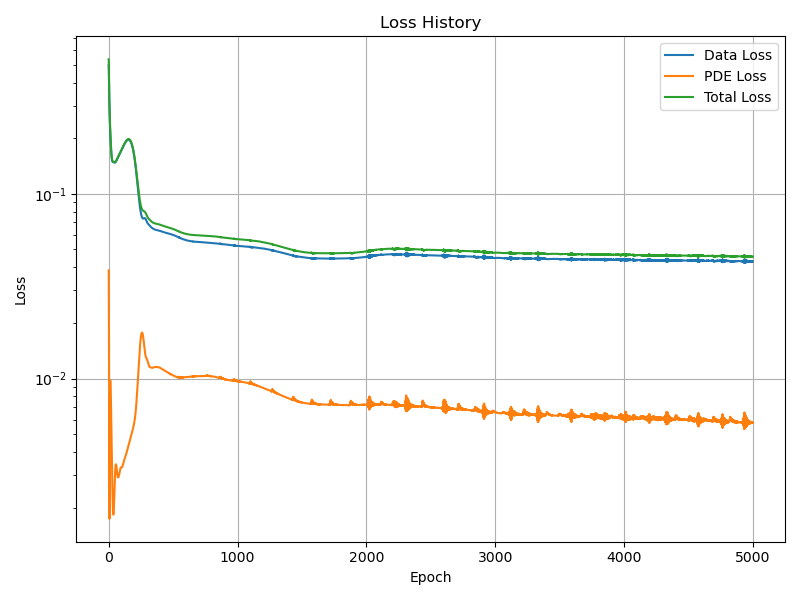
\includegraphics[width=0.6\textwidth]{1D_Loss_NU2_Annealing.png}
    \caption{Loss for Case 2: Low Viscosity}
    \label{fig:Loss_NU2_LR}
\end{figure}

Comparing the second case with and without learning rate annealing, the FFNN was yet again able to converge to a smoother loss function with less epochs. The data loss function converged to a value of $10^-1.5$ after approximately 2000 epochs.

\pagebreak
\subsubsection{Case 3: No Viscosity}
\begin{figure}[h!]
    \centering
    \begin{subfigure}[b]{0.48\textwidth}
        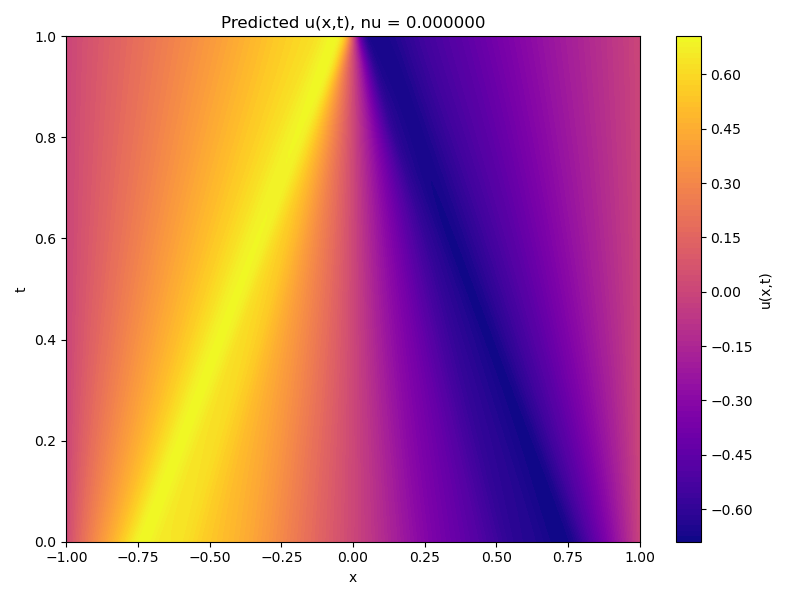
\includegraphics[width=\textwidth]{1D_PredGrad_NU3_Annealing.png}
        \caption{Prediction Gradient for Case 3: No Viscosity}
        \label{fig:PredGrad_NU3_LR}
    \end{subfigure}
    \hfill
    \begin{subfigure}[b]{0.48\textwidth}
        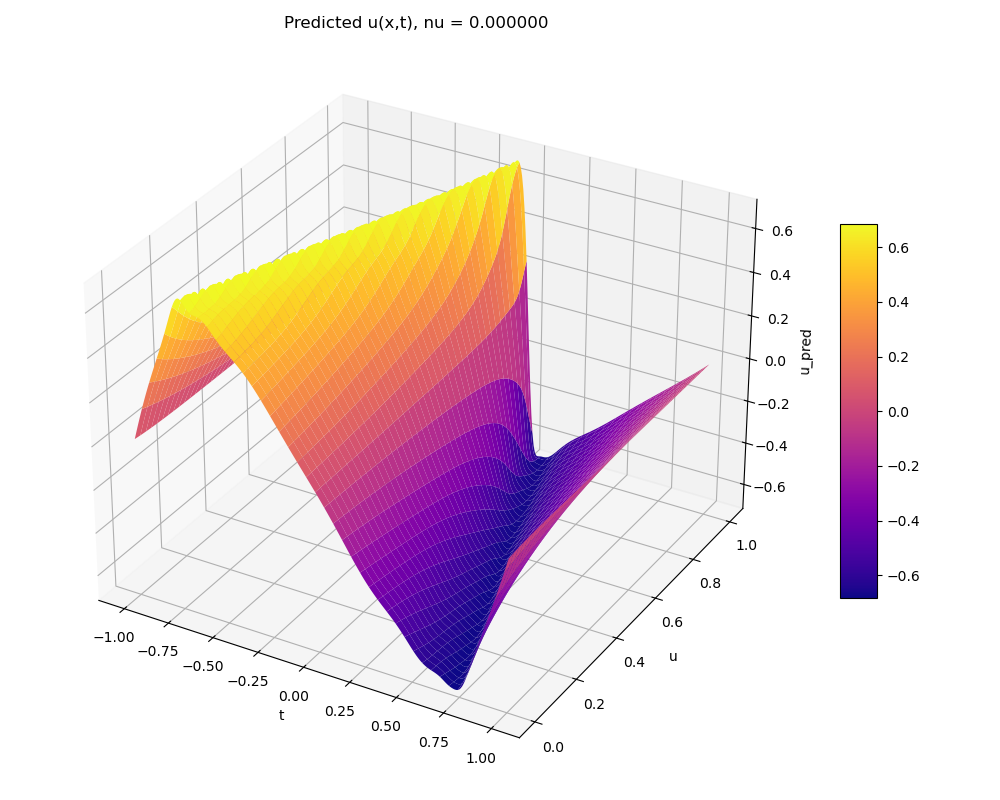
\includegraphics[width=\textwidth]{1D_Pred_NU3_Annealing.png}
        \caption{Prediction for Case 3: No Viscosity}
        \label{fig:Pred_NU3_LR}
    \end{subfigure}
    \caption{Prediction for Case 3: No Viscosity}
    \label{fig:PredTotal_NU3_LR}
\end{figure}
\begin{figure}[h]
    \centering
    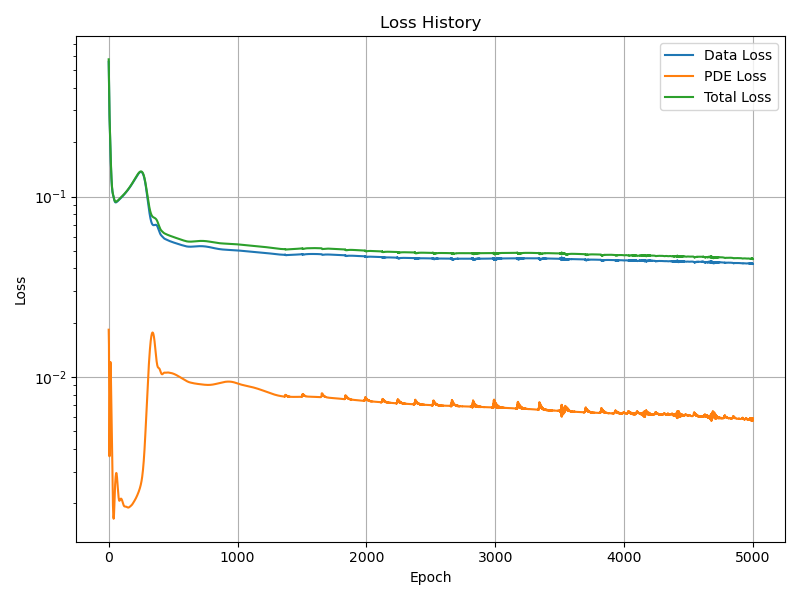
\includegraphics[width=0.6\textwidth]{1D_Loss_NU3_Annealing.png}
    \caption{Loss for Case 3: No Viscosity}
    \label{fig:Loss_NU3_LR}
\end{figure}

Comparing the third case with and without learning rate annealing, yet again the FFNN was able to converge to a smoother loss function with less epochs. The data function converged to a value of $10^-1.5$ after approximately 2500 epochs.

\subsection{Conclusion}

Overall, the FFNN was able to learn the underlying physics of the system and make accurate predictions based on the PDE and boundary conditions. The use of learning rate annealing significantly improved the speed of convergence and the smoothness of the loss function. Comparing to a numerical solution, the FFNN performed well and was able to capture the jump discontinuity in the viscous case.

\pagebreak

\section{2D Wave Equation}
For this problem, the same domain as the previous case is used, but the wave equation is given by:
\begin{equation}
    u_{tt} = c^2 (u_{xx} + u_{yy})
\end{equation}
where $c$ is the wave speed. The closed form solution is given by:
\begin{equation}
    u(x, y, t) = \sin(k \pi x) \sin(k \pi y) \cos(\omega t) 
\end{equation}
where $k$ is the wave number and $\omega$ is the angular frequency given by:
\begin{equation}
    \omega = \sqrt{2} c \pi k
\end{equation}

The following parameters are used for the 2D wave equation:
\begin{itemize}
    \item k = $\lbrace 2, 10, 25 \rbrace$
    \item Epochs = 10000
    \item LearningRate = $5 \cdot 10^{-4}$
    \item Neurons = 50
    \item $N_{i}  = 5000$ (interior points)
    \item $N_{b}  = 256$  (boundary points)
    \item $N_{ic} = 256$  (initial condition points)
    \item $N_{bc} = 256$  (boundary condition points)
\end{itemize}

The NN will be trained on the interior points, boundary points and initial conditions. For the wave equation, since the closed form solution is known, the loss function is defined by:
\begin{equation}
    L = L_{pde} + L_{ic} + L_{bc}
\end{equation}

where,
\begin{equation}
    L_{pde} = u_{tt} - c^2 (u_{xx} + u_{yy})
\end{equation}

\begin{equation}
    L_{ic} = \frac{1}{N} \sum_{i=1}^{N} (\theta(u|x_{ic}, y_{ic}, t_{ic})-u_{ic})^2
\end{equation}
\begin{equation}
    L_{bc} = \frac{1}{N} \sum_{i=1}^{N} (\theta(u|x_{bc}, y_{bc}, t_{bc})-u_{bc})^2
\end{equation}

\pagebreak
\subsection{Results - Tanh Activation}

\begin{figure}[h!]
    \centering
    \begin{subfigure}[b]{0.48\textwidth}
        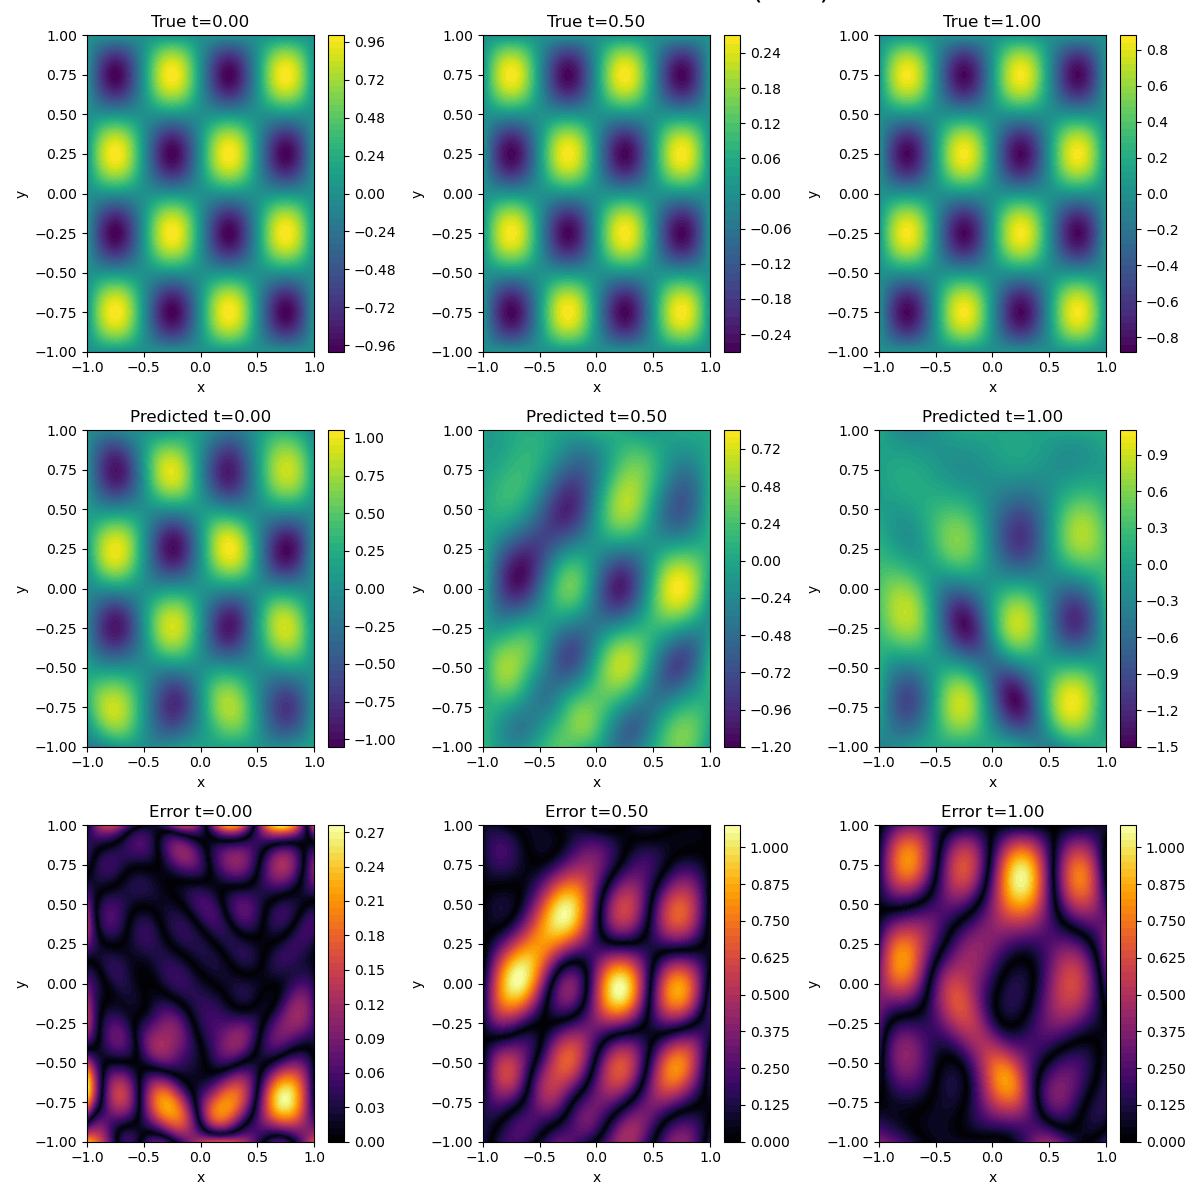
\includegraphics[width=\textwidth]{2D_Error_K1.png}
        \caption{Error for Case 1: k = 2}
        \label{fig:Error_K1}
    \end{subfigure}
    \hfill
    \begin{subfigure}[b]{0.48\textwidth}
        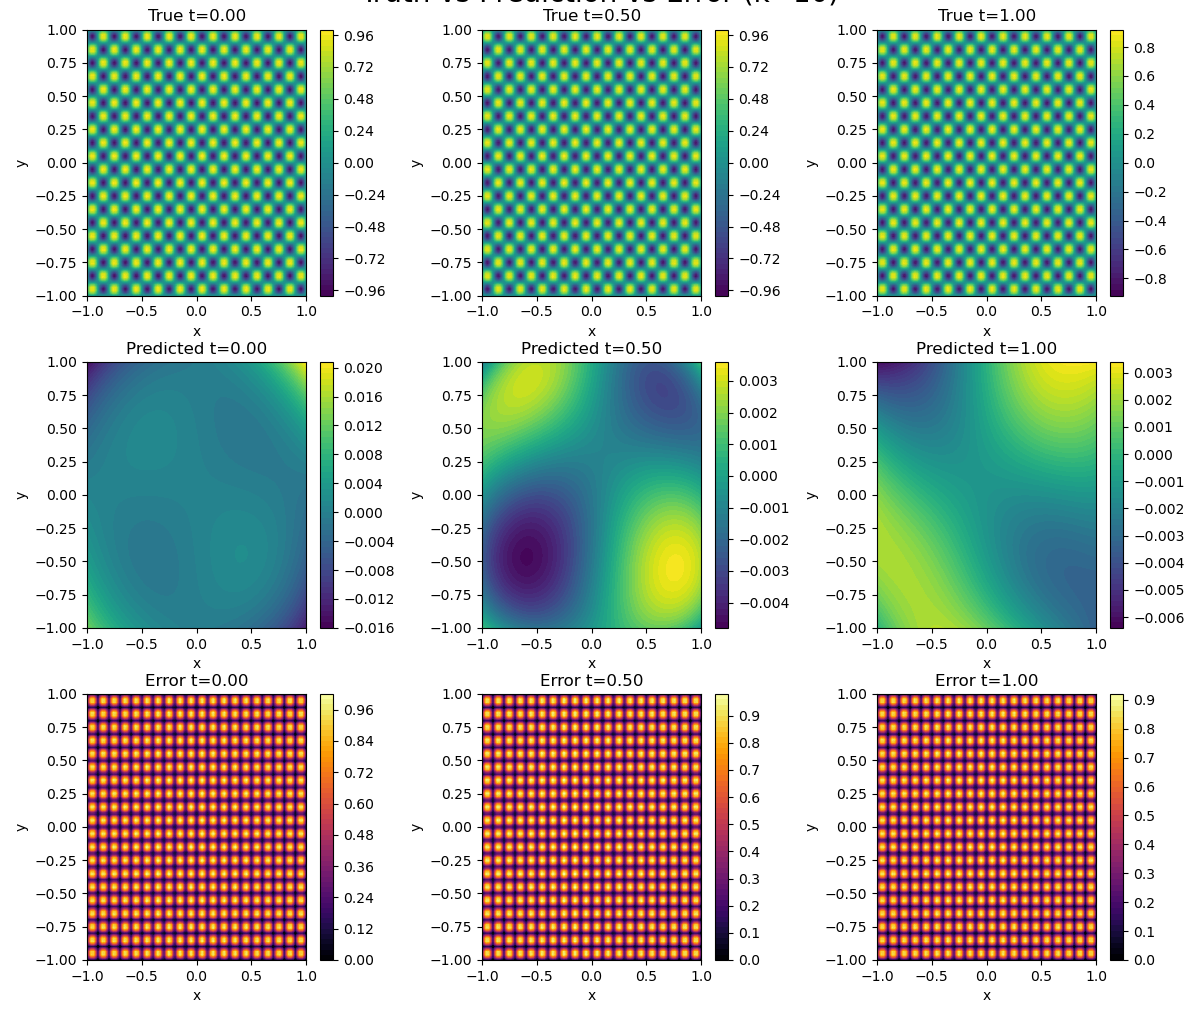
\includegraphics[width=\textwidth]{2D_Error_K2.png}
        \caption{Error for Case 2: k = 10}
        \label{fig:Error_K2}
    \end{subfigure}
    \hfill
    \begin{subfigure}[b]{0.48\textwidth}
        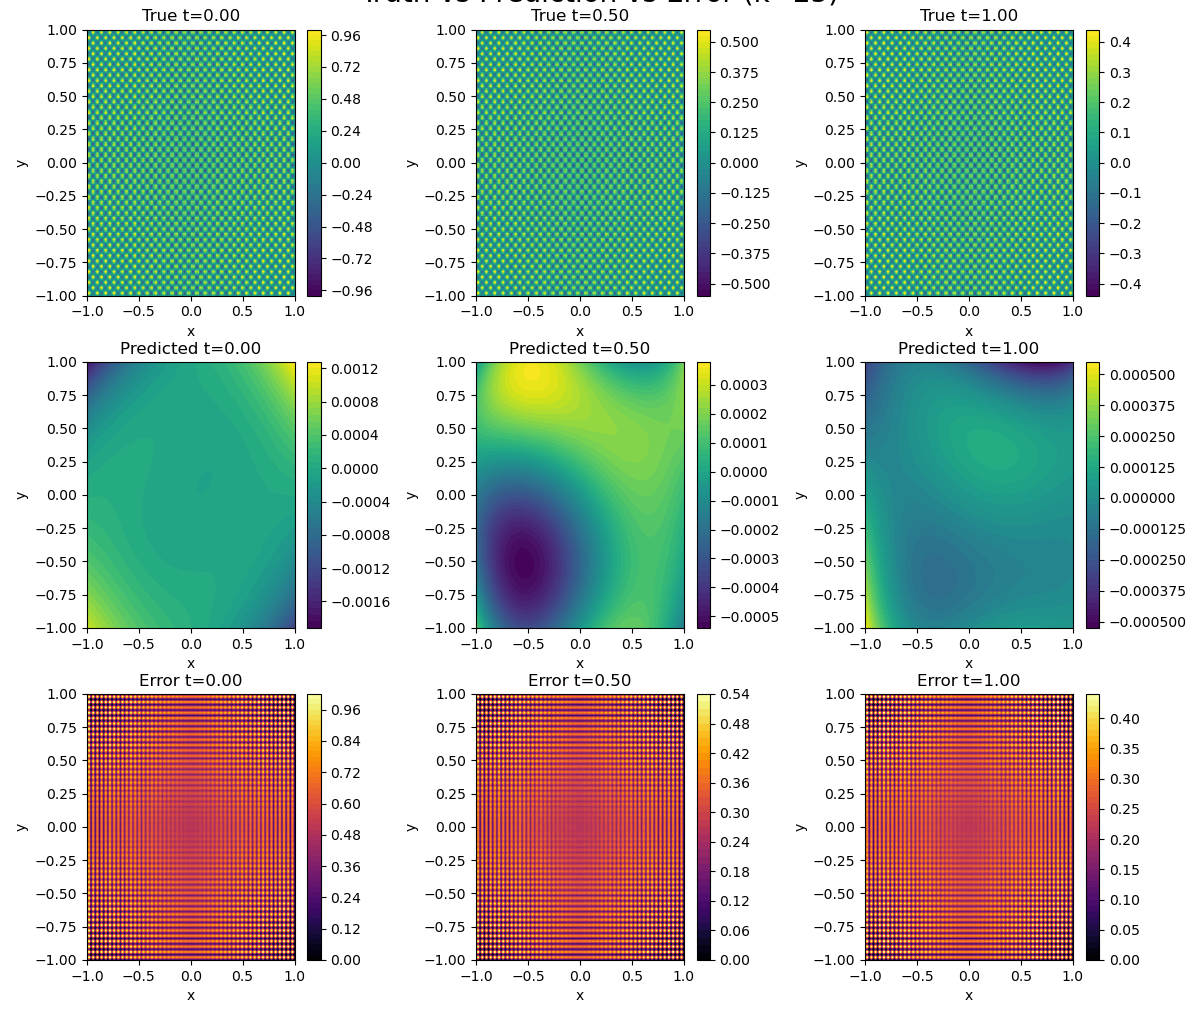
\includegraphics[width=\textwidth]{2D_Error_K3.png}
        \caption{Error for Case 3: k = 25}
        \label{fig:Error_K3}
    \end{subfigure}
    \caption{Error using Tanh Activation}
    \label{fig:Error_Tanh}
\end{figure}
\pagebreak

\begin{figure}[h!]
    \centering
    \begin{subfigure}[b]{0.48\textwidth}
        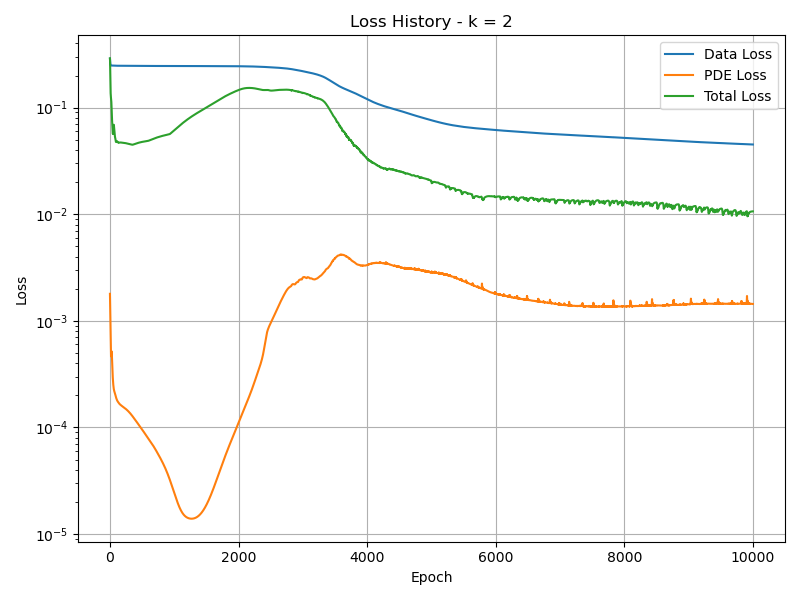
\includegraphics[width=\textwidth]{2D_Loss_K1.png}
        \caption{Loss for Case 1: k = 2}
        \label{fig:Loss_K1}
    \end{subfigure}
    \hfill
    \begin{subfigure}[b]{0.48\textwidth}
        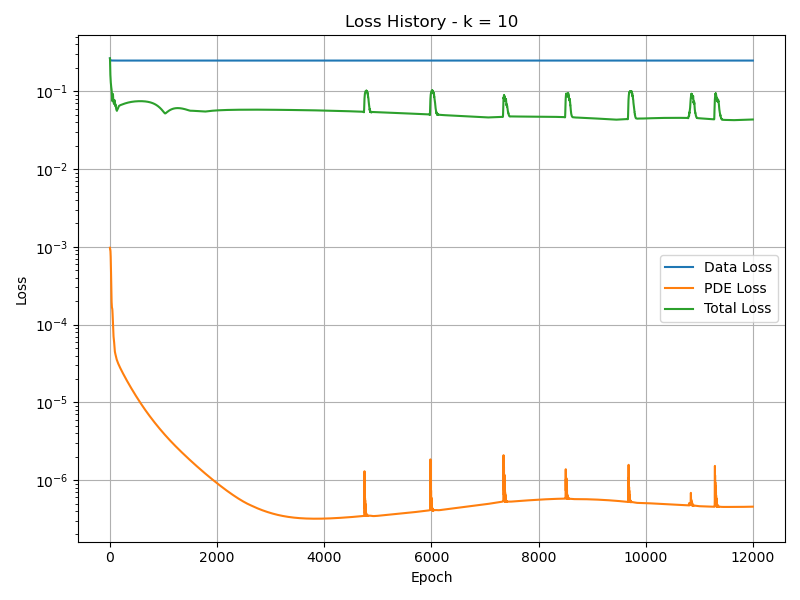
\includegraphics[width=\textwidth]{2D_Loss_K2.png}
        \caption{Loss for Case 2: k = 10}
        \label{fig:Loss_K2}
    \end{subfigure}
    \hfill
    \begin{subfigure}[b]{0.48\textwidth}
        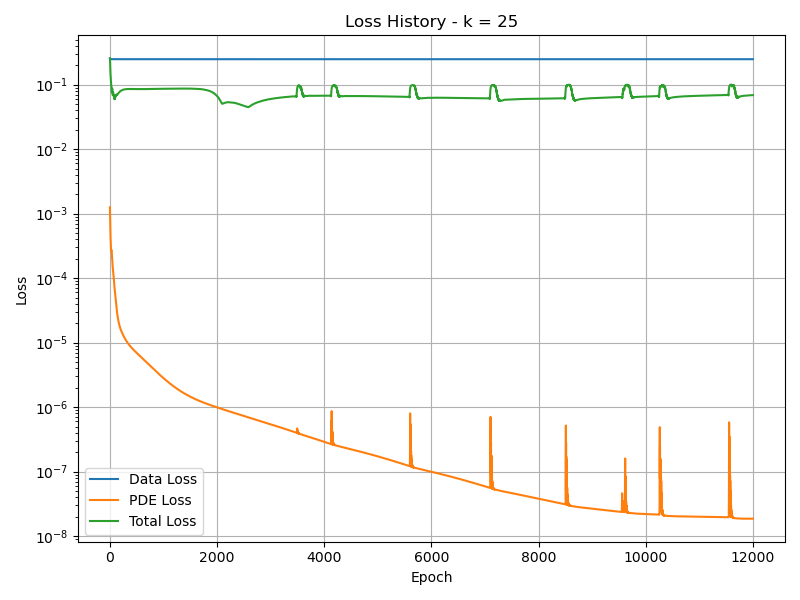
\includegraphics[width=\textwidth]{2D_Loss_K3.png}
        \caption{Loss for Case 3: k = 25}
        \label{fig:Loss_K3}
    \end{subfigure}
    \caption{Loss Function using Tanh Activation}
    \label{fig:Loss_Tanh}
\end{figure}
\pagebreak

\begin{figure}[h!]
    \centering
    \begin{subfigure}[b]{0.48\textwidth}
        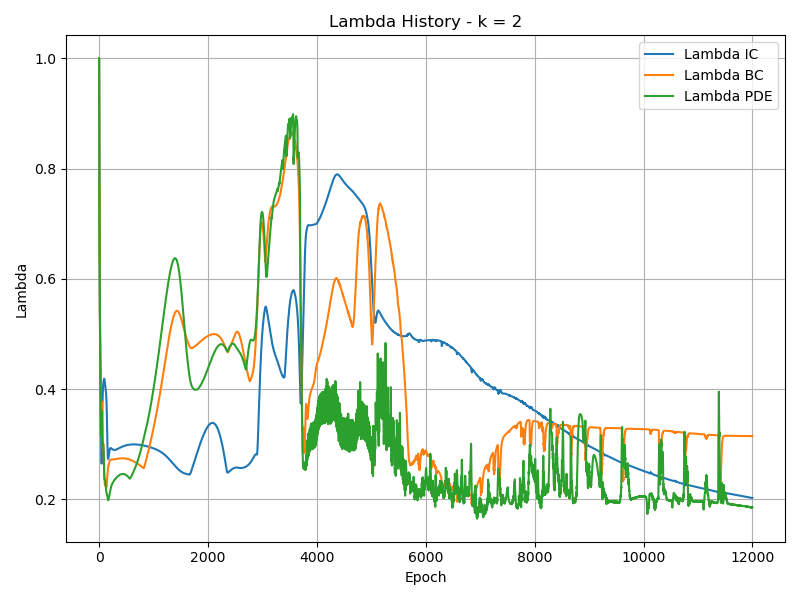
\includegraphics[width=\textwidth]{2D_Lambda_K1.png}
        \caption{Lambda for Case 1: k = 2}
        \label{fig:Lambda_K1}
    \end{subfigure}
    \hfill
    \begin{subfigure}[b]{0.48\textwidth}
        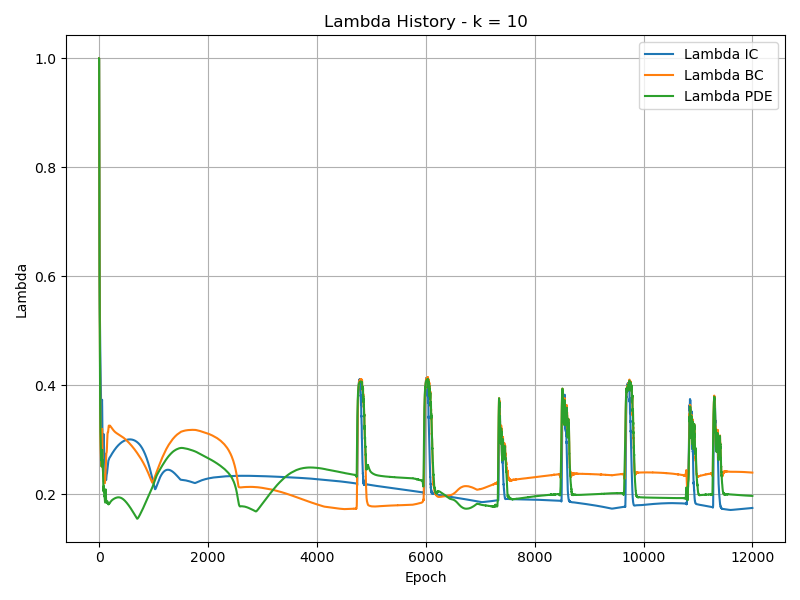
\includegraphics[width=\textwidth]{2D_Lambda_K2.png}
        \caption{Lambda for Case 2: k = 10}
        \label{fig:Lambda_K2}
    \end{subfigure}
    \hfill
    \begin{subfigure}[b]{0.48\textwidth}
        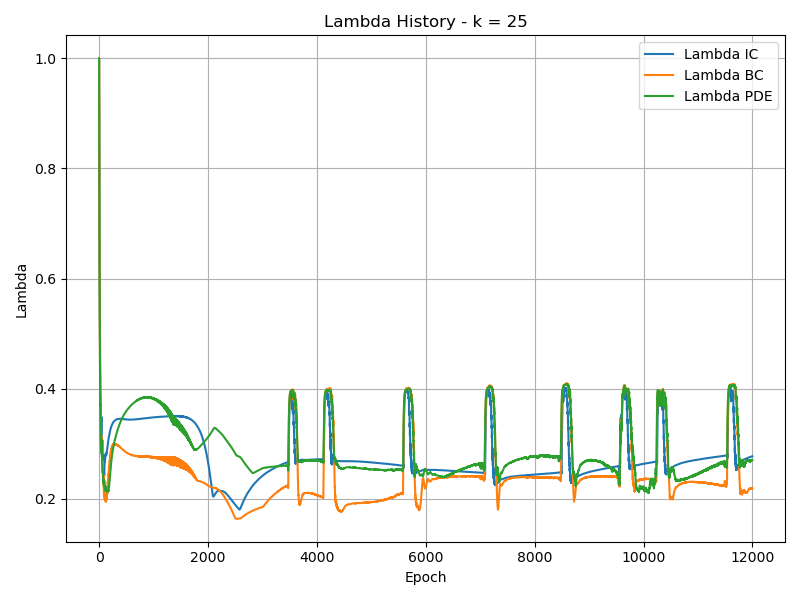
\includegraphics[width=\textwidth]{2D_Lambda_K3.png}
        \caption{Lambda for Case 3: k = 25}
        \label{fig:Lambda_K3}
    \end{subfigure}
    \caption{Lambda for Case 3: No Viscosity}
    \label{fig:Lambda_Tanh}
\end{figure}

For the 2D wave equation, the FFNN was able to learn the underlying physics of the first case where $k=2$ decently well. The loss function converged to a value of $10^{-2}$. The prediction gradient and error plot in Figure~\ref{fig:Error_Tanh} show that the prediction matches the initial conditions and boundary conditions well. As time progresses, the prediction becomes less accurate but still captures the expected behavior of the wave equation.

As the wave number increases, the FFNN has a harder time learning the underlying physics of the system. For both the $k=10$ and $k=25$ cases, the FFNN converged to a loss of $10^{-1.2}$. The prediction gradient and error plot in Figure~\ref{fig:Error_Tanh} show that the prediction does not match the initial conditions but does match the boundary conditions. With this, the PDE loss is very low compared to the data loss. The error seen in the prediction is likely due to the fact that the wave number is too high for the FFNN to learn the initial conditions well enough.

Without the initial conditions, the FFNN will not be able to learn the underlying physics of the system at all. The start conditions can be thought of as the initial velocity of the wave. That wave behaves differently depending on the initial velocity and cannot be learned without it. Shown in the loss function, the initial conditions loss converges to a value of exactly 0.2480 for both the $k=10$ and $k=25$ cases and the PDE loss converges to a value of $10^{-6.4}$ and $10^{-7.8}$ respectively. 

\subsection{Results - Rowdy Activation}
Since the traditional tanh activation function did not perform well for the 2D wave equation, a new activation function was considered. The Rowdy Activation Function (Deep Kronecker neural network) is given by:
\begin{equation}
    \phi_1 = \frac{e^z-e^{-z}}{e^z+e^{-z}} \equiv \tanh(z)
\end{equation}
\begin{equation}
    \phi_2 = n a \sin((k-1)n x)
\end{equation}
\begin{equation}
    \phi_3 = n b \sin((k-1)n x)
\end{equation}

\begin{figure}[h!]
    \centering
    \begin{subfigure}[b]{0.48\textwidth}
        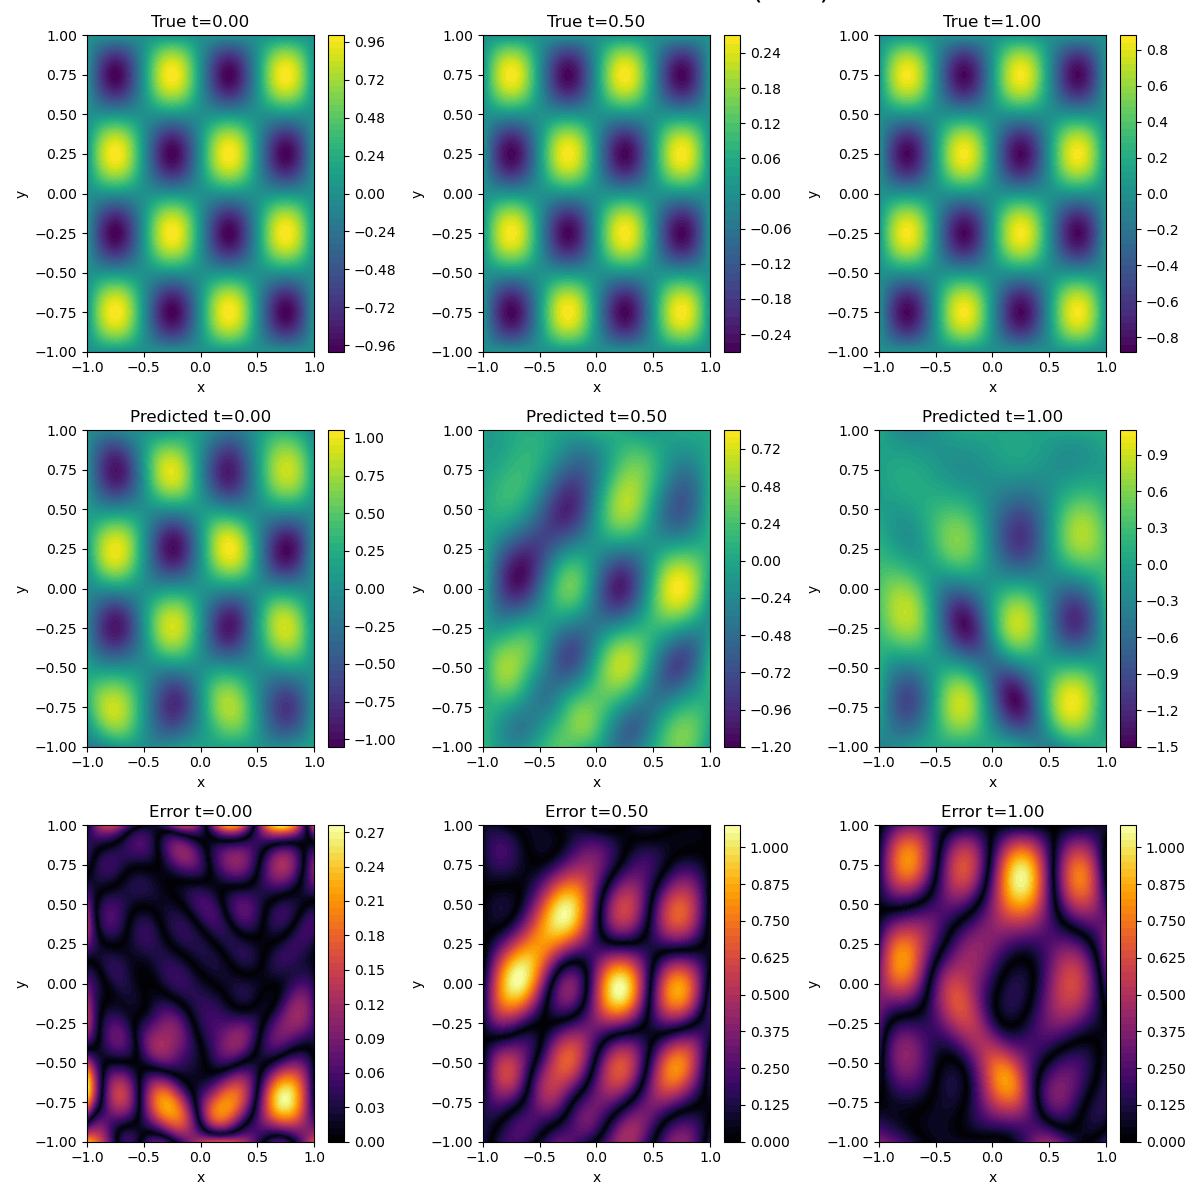
\includegraphics[width=\textwidth]{2D_Error_K1_Rowdy.png}
        \caption{Error for Case 1: k = 2}
        \label{fig:Error_K1_Rowdy}
    \end{subfigure}
    \hfill
    \begin{subfigure}[b]{0.48\textwidth}
        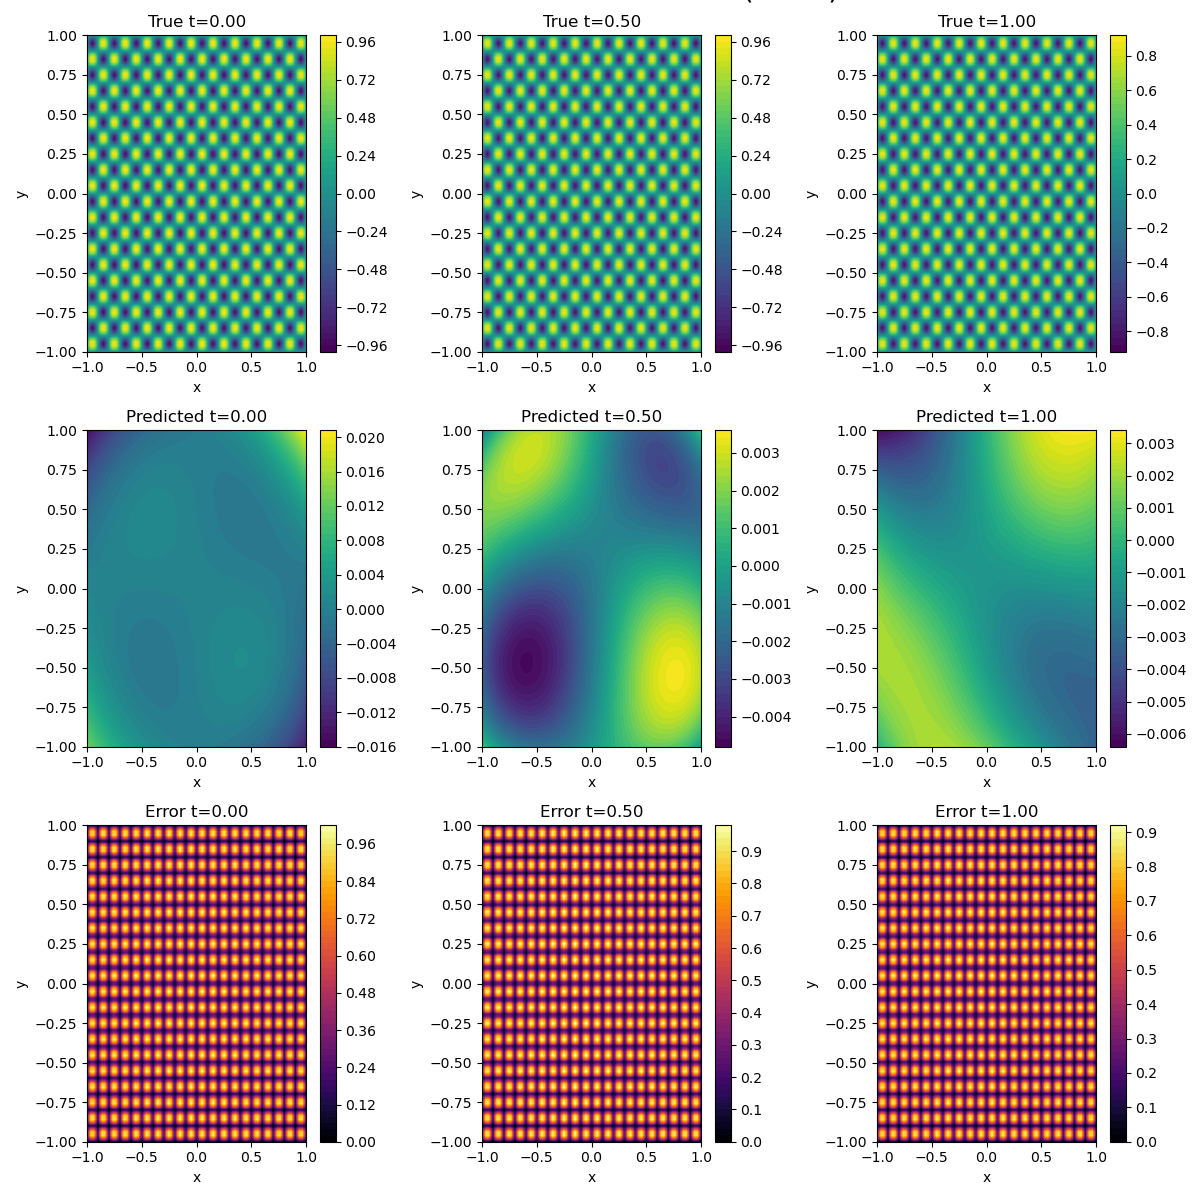
\includegraphics[width=\textwidth]{2D_Error_K2_Rowdy.png}
        \caption{Error for Case 2: k = 10}
        \label{fig:Error_K2_Rowdy}
    \end{subfigure}
    \hfill
    \begin{subfigure}[b]{0.48\textwidth}
        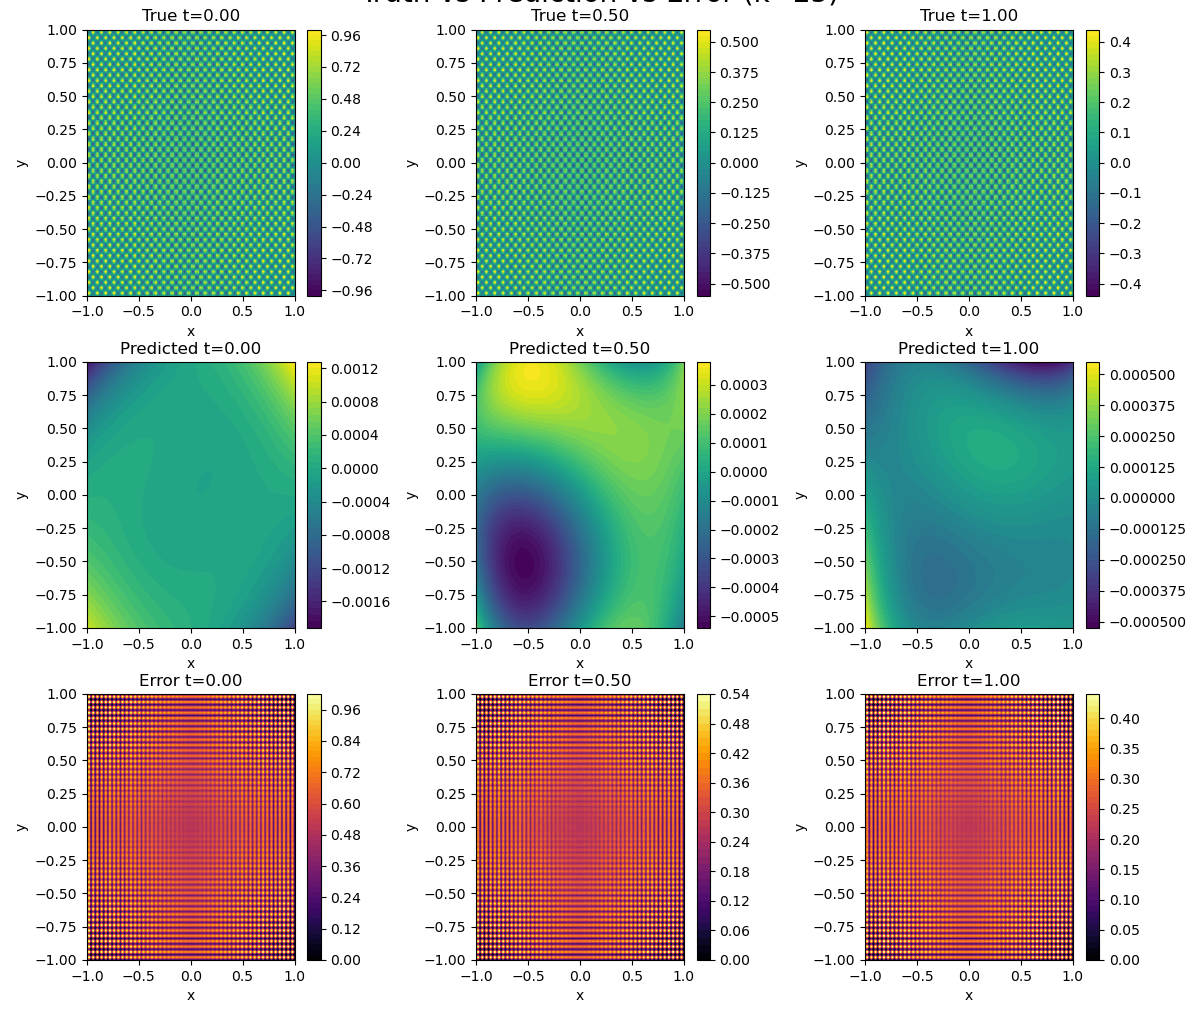
\includegraphics[width=\textwidth]{2D_Error_K3.png}
        \caption{Error for Case 3: k = 25}
        \label{fig:Error_K3_Rowdy}
    \end{subfigure}
    \caption{Error using Rowdy Activation}
    \label{fig:Error_Rowdy}
\end{figure}
\pagebreak

\begin{figure}[h!]
    \centering
    \begin{subfigure}[b]{0.48\textwidth}
        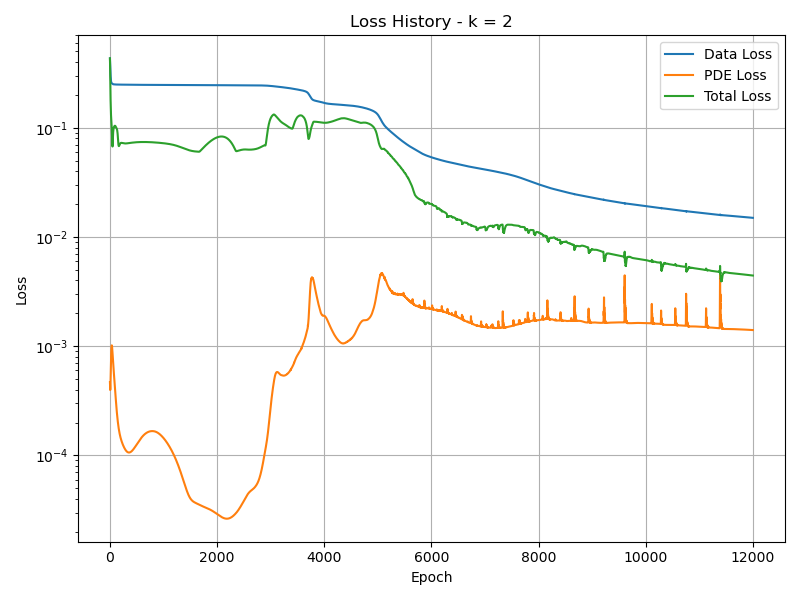
\includegraphics[width=\textwidth]{2D_Loss_K1_Rowdy.png}
        \caption{Loss for Case 1: k = 2}
        \label{fig:Loss_K1_Rowdy}
    \end{subfigure}
    \hfill
    \begin{subfigure}[b]{0.48\textwidth}
        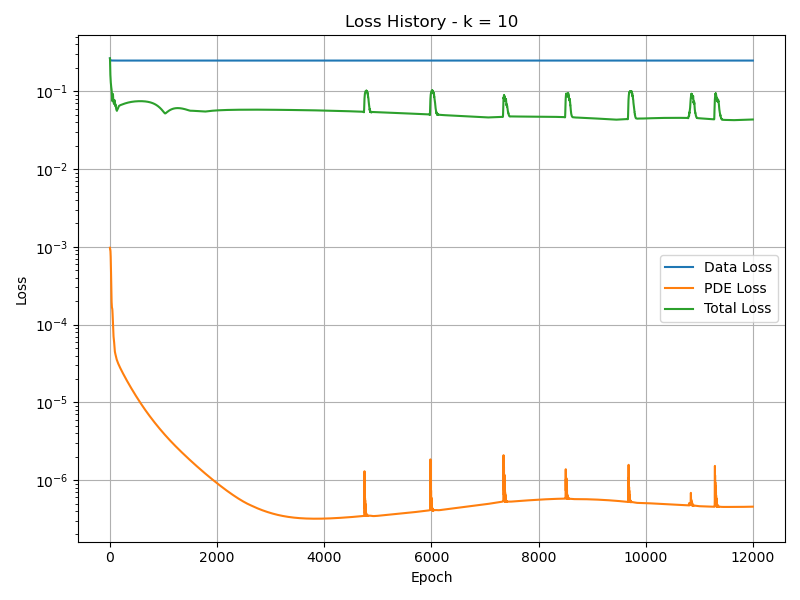
\includegraphics[width=\textwidth]{2D_Loss_K2_Rowdy.png}
        \caption{Loss for Case 2: k = 10}
        \label{fig:Loss_K2_Rowdy}
    \end{subfigure}
    \hfill
    \begin{subfigure}[b]{0.48\textwidth}
        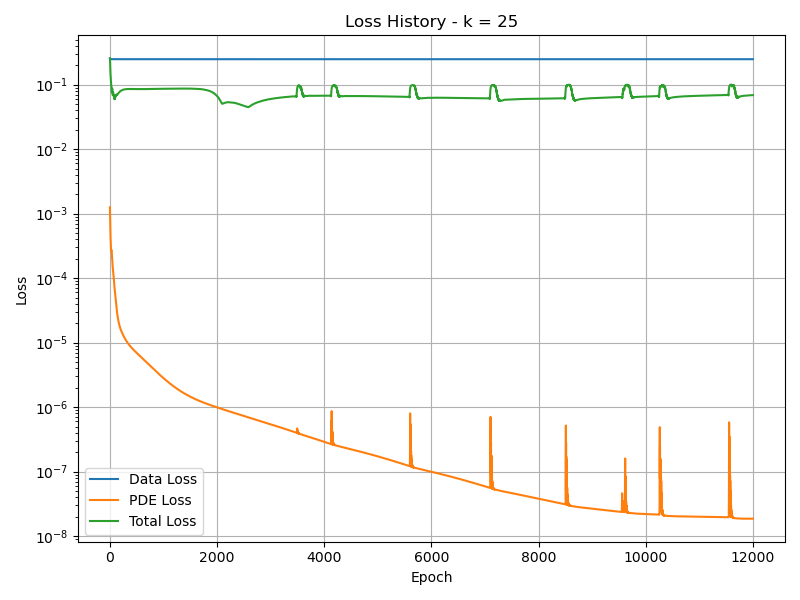
\includegraphics[width=\textwidth]{2D_Loss_K3.png}
        \caption{Loss for Case 3: k = 25}
        \label{fig:Loss_K3_Rowdy}
    \end{subfigure}
    \caption{Loss Function using Rowdy Activation}
    \label{fig:Loss_Rowdy}
\end{figure}
\pagebreak

\begin{figure}[h!]
    \centering
    \begin{subfigure}[b]{0.48\textwidth}
        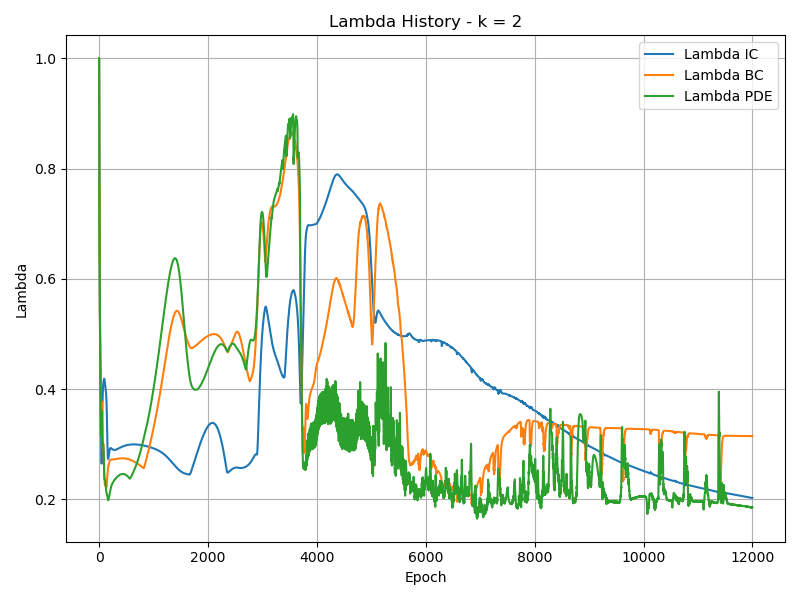
\includegraphics[width=\textwidth]{2D_Lambda_K1_Rowdy.png}
        \caption{Loss for Case 1: k = 2}
        \label{fig:Lambda_K1_Rowdy}
    \end{subfigure}
    \hfill
    \begin{subfigure}[b]{0.48\textwidth}
        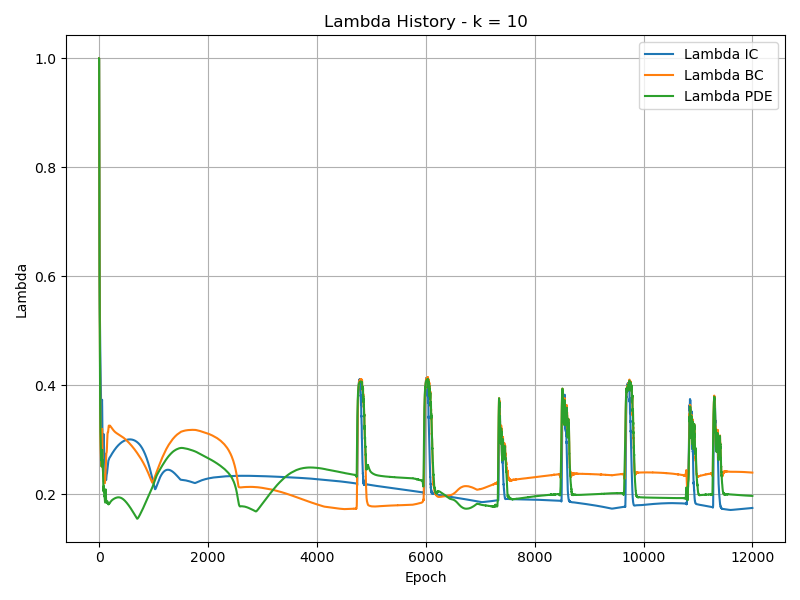
\includegraphics[width=\textwidth]{2D_Lambda_K2_Rowdy.png}
        \caption{Loss for Case 2: k = 10}
        \label{fig:Lambda_K2_Rowdy}
    \end{subfigure}
    \hfill
    \begin{subfigure}[b]{0.48\textwidth}
        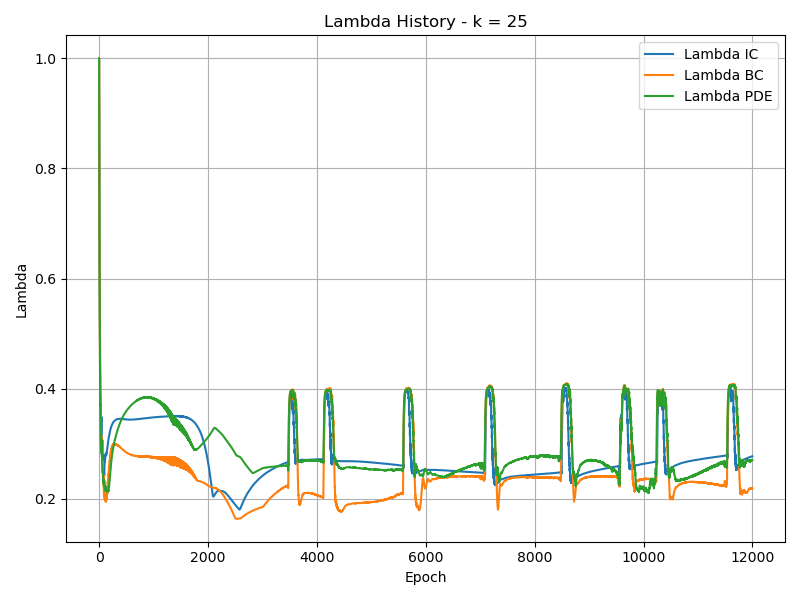
\includegraphics[width=\textwidth]{2D_Lambda_K3.png}
        \caption{Loss for Case 3: k = 25}
        \label{fig:Lambda_K3_Rowdy}
    \end{subfigure}
    \caption{Lambda using Rowdy Activation}
    \label{fig:Lambda_Rowdy}
\end{figure}

Using the Rowdy activation function, the FFNN was able to achieve slightly better results for case 1 with $k=2$. The loss function reached a value of $10^{-2.5}$ and still descending. Given more epochs, the FFNN would likely converge to a lower loss function but from this point was a relatively small gradient. The prediction and error plot in Figure~\ref{fig:Error_Rowdy} show that the prediction matches the initial conditions and boundary conditions well. Unlike the tanh activation function, the Rowdy activation function was able to learn the initial conditions well and through the entire domain. 

Despite the better results for case 1, the FFNN still was unable to learn the underlying physics of the system for the $k=10$ and $k=25$ cases. Yet again, the initial conditions are still converging to a value of eitherr 0.2480 or 0.2490. The PDE loss is still very low compared to the data loss. Using the Rowdy activation function, the PDE loss converged to a value less than that of the tanh activation function.

\section{Conclusion}
In this assignment, a FFNN was trained on the 1D viscous Burgers equation as well as the 2D wave equation. While the FFNN did a good job learning the 1D viscous Burgers equation, it clearly struggled with the higher wave numbers in the 2D wave function. This assignment was a great introduction to the use of PINNs and provided a great baseline for future work into the final project. Even for the 1D viscous Burgers equation, where the exact closed form solution is not known, the PINN was able to learn the equation well and provide an approximation comparable to a traditional numerical solution. The use of learning rate annealing proved to be very useful in faster convergence and left all cases with a smoother loss function.

Despite the success of the PINN for the 1D viscous Burgers equation and Case 1 of the 2D wave equation, the PINN still struggled with the higher wave numbers. The use of the Rowdy activation function did help with the convergence of the loss function but still did not improve the solution for the higher wave numbers. Still the major issue with the PINN is the significant dependence on the initial conditions. Without the initial conditions, the PINN will not be able to learn the full phyiscs of the system. This is true for all PDEs and even effects numerical solutions, not just PINNs, but this particular case is very sensitive to the initial conditions - unveiling the limitations of the PINN approach. Potential future work could include the use of a different base activation function, a different loss function, or further tunning of the hyperparameters despite current efforts returning no significant improvements.

\newpage
\section{1dBurgers.py}
\lstinputlisting[language=python]{1dBurgers.py}

\newpage
\section{2dWave.py}
\lstinputlisting[language=python]{2dwave.py}

\end{document}